\documentclass[a4j,pt]{jsarticle}
\usepackage{layout,url,resume}
\usepackage[dvipdfmx]{graphicx}
\pagestyle{empty}

\begin{document}
%\layout

\title{Hogehoge \\ fugafuga}

% 和文著者名
\author{
   Tomoya Iwasaki 
}

% 和文概要
\begin{abstract}
hogehoge
\end{abstract}

\maketitle
\thispagestyle{empty}

\section{はじめに}
hogehoge


\section{背景}

\subsection{その1}

hogehoge\cite{example}
\begin{figure}[htbp]
    \begin{center}
        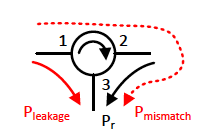
\includegraphics[width=6cm]{circulator.png}
        \caption{picture}
        \label{sample}
    \end{center}
\end{figure}

\subsection{その2}

\cite{example2}参考文献はこれ


%---------------------------------------------

\section{本手法}

\begin{figure}[htbp]
    \begin{center}
        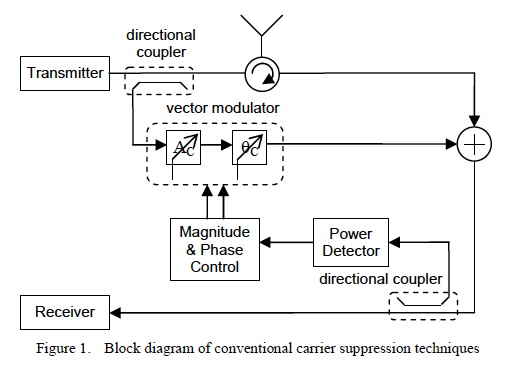
\includegraphics[width=6cm]{diagram_VectorModulation.png}
        \caption{picture2}
        \label{sample}
    \end{center}
\end{figure}


\bibliographystyle{junsrt}
\bibliography{resume}

\end{document}
% end of file
